\chapter{Handling Identification}

\section{Exercise 1 - Sine Steer Maneuvers}

\textbf{Q. Perform a set of sine steer maneuvers, with steering wheel angle $\deltd$\ = $\deltdz$\ $\sin(2\pi ft)$. Use $\deltdz$\ = $5^\circ$, and repeat the test at 3 different u = \{50, 80, 100\} km/h.}

        \begin{figure}[ht]
        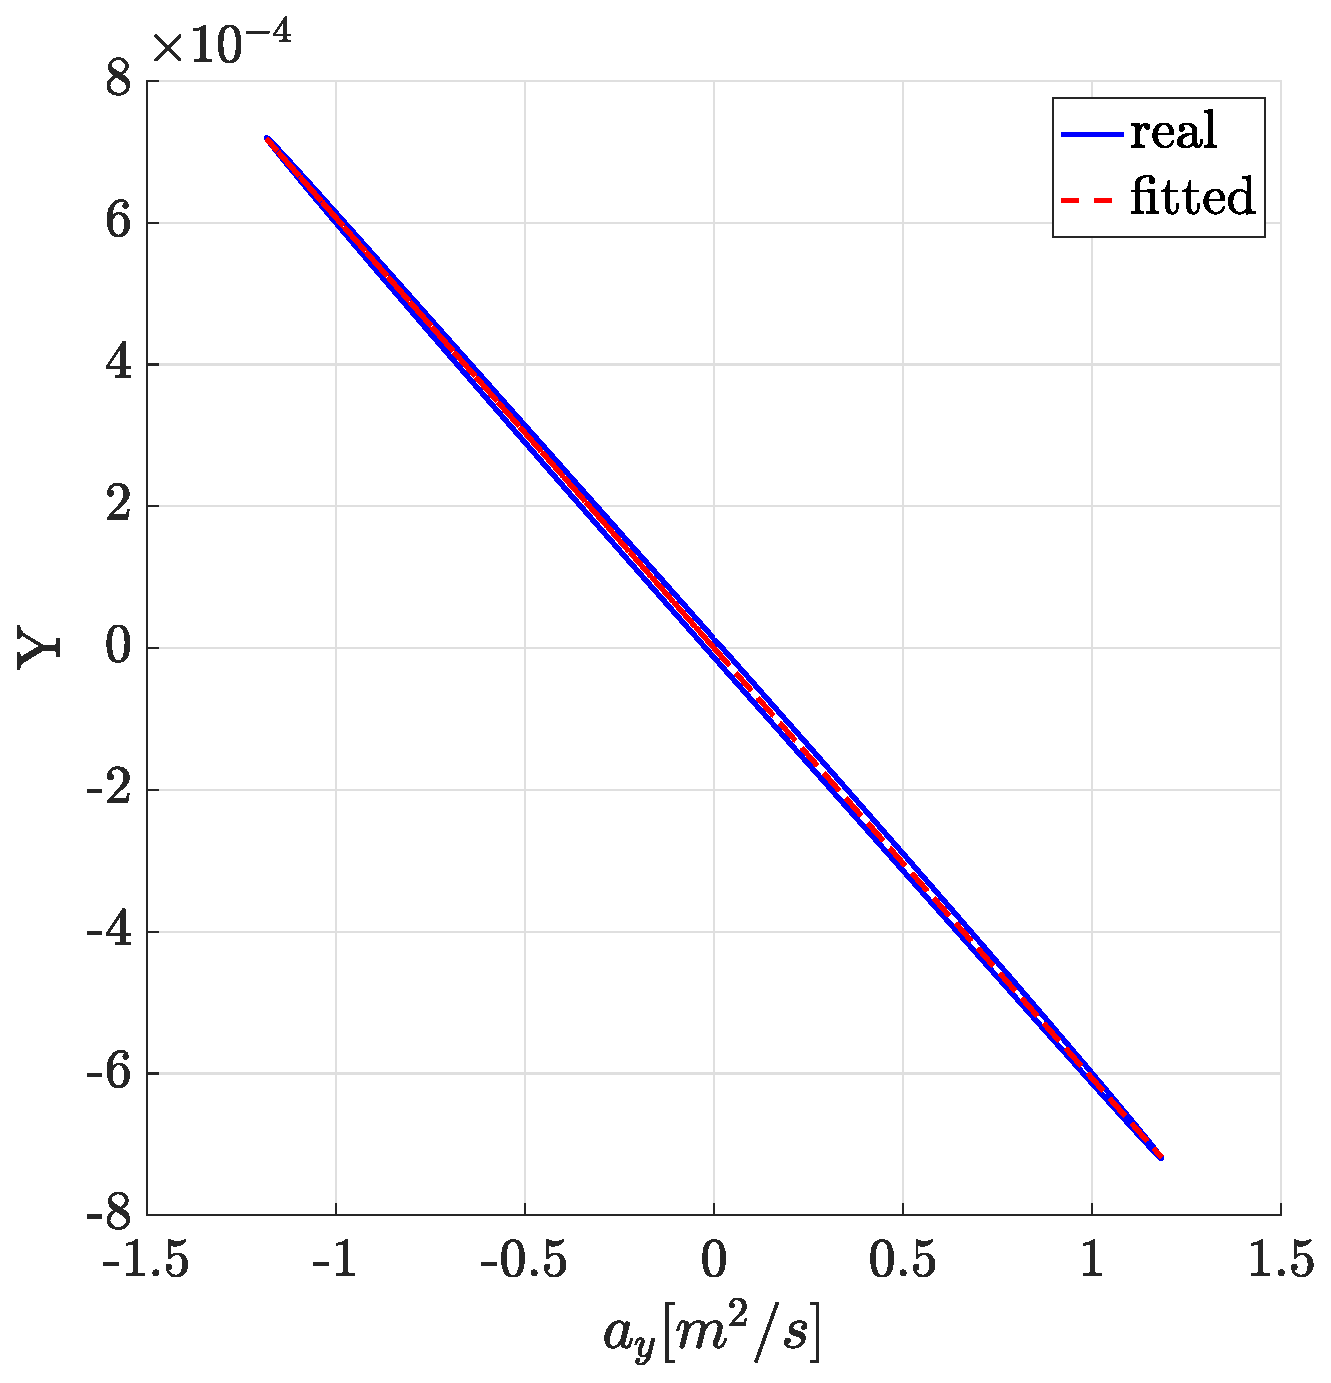
\includegraphics[width=0.5\linewidth]{ex5/q1/ex-51b1.eps}
        \centering
        \caption{Fitted handling diagram result [$\deltdz$\ = $5^\circ$, $u$ = 50 km/h]}
        \label{51b1}
        \end{figure}

Figure \ref{51b1} shows the handling diagram result of a sine steering maneuver that uses a desired steering angle $\deltd$\ = $\deltdz$\ $\sin(2\pi ft)$ at speed 50 km/h. The frequency $f$ in the equation is the number of complete cycles that happen every second. We must perform changes to our system very slowly in order to preserve steady state conditions. The frequency used was $0.001$ $s^{-1}$ and the simulation time was 1000 seconds. The  Y refers to the handling behaviour of the vehicle and is calculated using Equation \ref{eq:5.1}:

\begin{equation}\label{eq:5.1}
    Y = \delta - \frac{\Omega}{u} L
\end{equation}

The handling curve obtained at 50 km/h has a negative slope and appears to be linear. The data can be fitted with a first degree polynomial [$f(x) = ax +b$] as shown in Figure \ref{51b1}.

The negative slope indicates that the vehicle exhibits an over-steering behaviour. Over-steering occurs when the vehicle's rear wheels have higher lateral slip compared to the front [$\alpha_{r} > \alpha_{f}$]. This causes the rear wheels to have a larger radius of curvature than the front and the vehicle steers more than expected. If we want to keep the same radius of curvature in an over-steering condition, we must decrease the steering angle $\delta$ at higher velocities.

        \begin{figure}[ht]
        \includegraphics[width=0.99\linewidth]{ex5/q1/ex-51c.eps}
        \centering
        \caption{Handling diagram results at different speeds with same $\deltd$}
        \label{51c}
        \end{figure}

The slope of the line represents the under-steering gradient $\kus$. It describes the evolution of $\delta$ as $\ay$ increases. $\kus$ is positive if the vehicle is under-steering and negative when over-steering.

Increasing the speeds to 80 and 100 km/h resulted in an increase in the lateral acceleration $\ay$ as shown in Figure \ref{51c}. The vehicle nonetheless showed over-steering behaviour across all the simulated speeds. A comparison between the yaw-rate $\Omega$ and the desired steering angle $\deltd$ shows that the $\Omega$ keeps increasing with higher speeds while $\deltd$ does not.

        \begin{figure}[ht]
        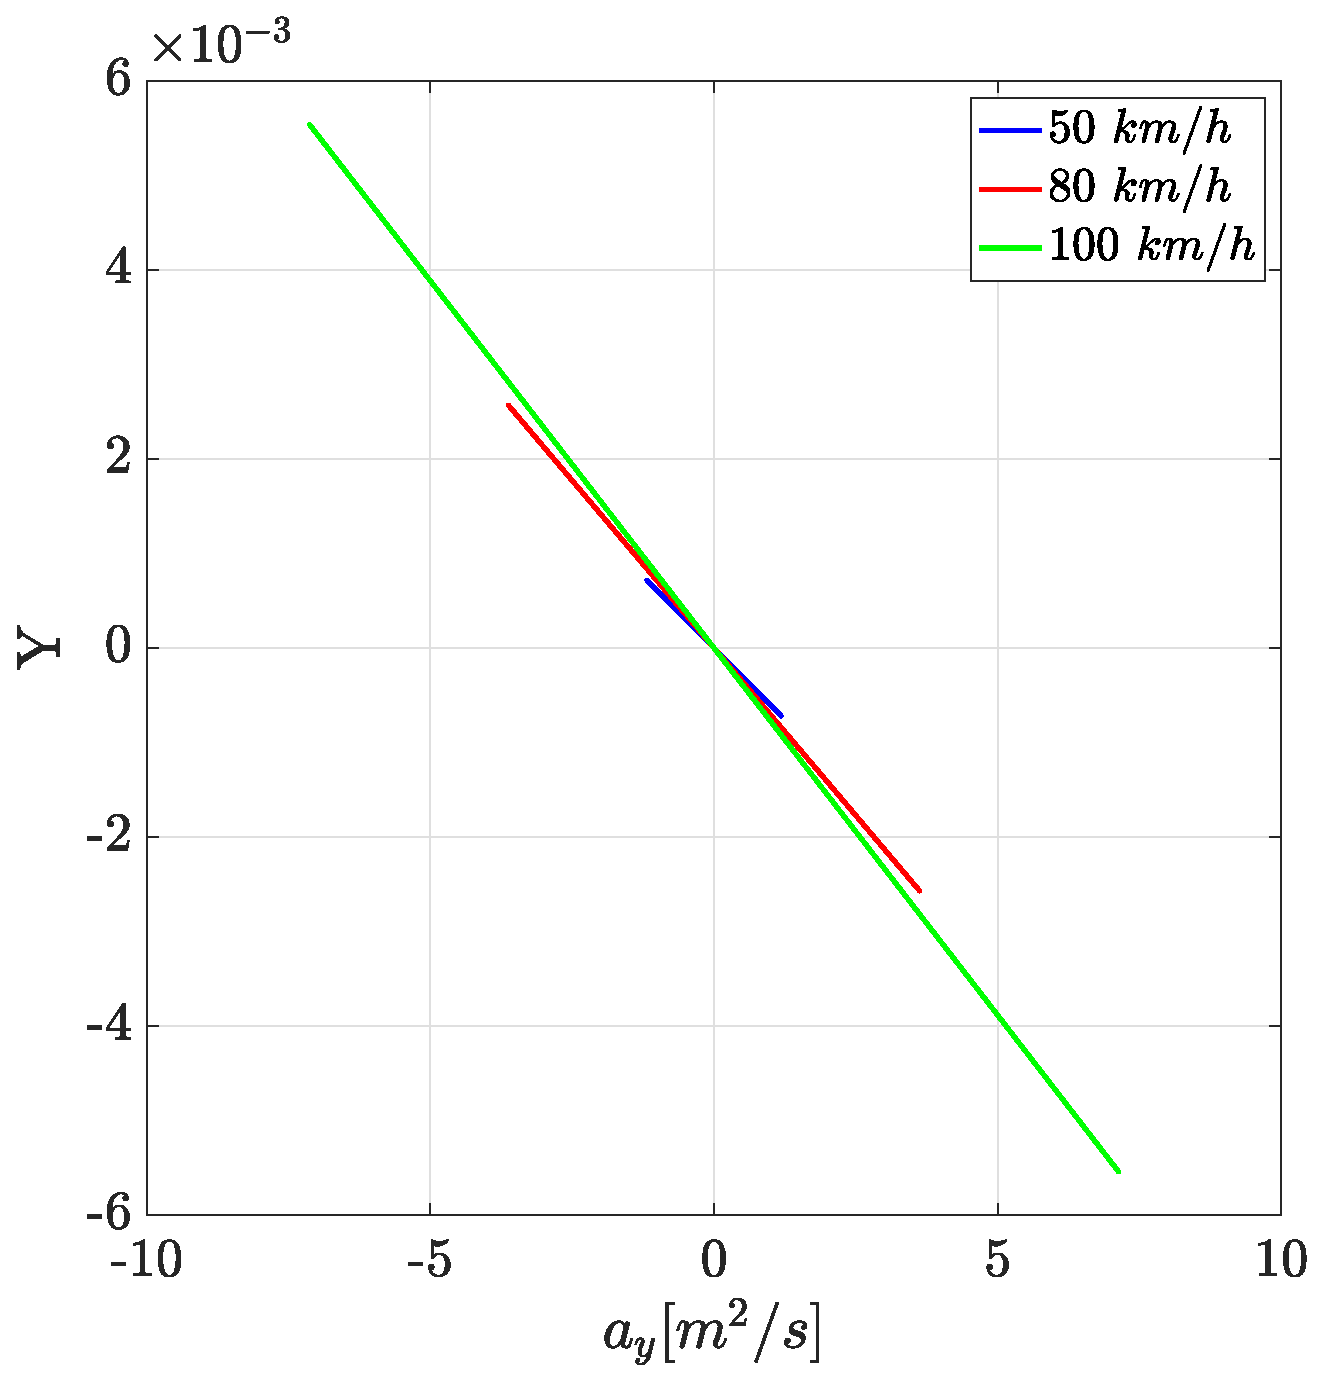
\includegraphics[width=0.75\linewidth]{ex5/q1/ex-51d.eps}
        \centering
        \caption{Fitted handling curves comparison with same $\deltd$}
        \label{51d}
        \end{figure}
        
Superimposing the handling curves of the three simulated speeds in Figure \ref{51d} clearly shows that with higher speeds, the over-steering behavior increases [steeper negative slope]. That means $\delta$ will need to be decreased even further with higher speeds to keep the same curvature. Furthermore, the obtained curves pass through the origin. That means when there is no lateral acceleration $\ay$, the steering behaviour will be neutral. 

        \begin{figure}[ht]
        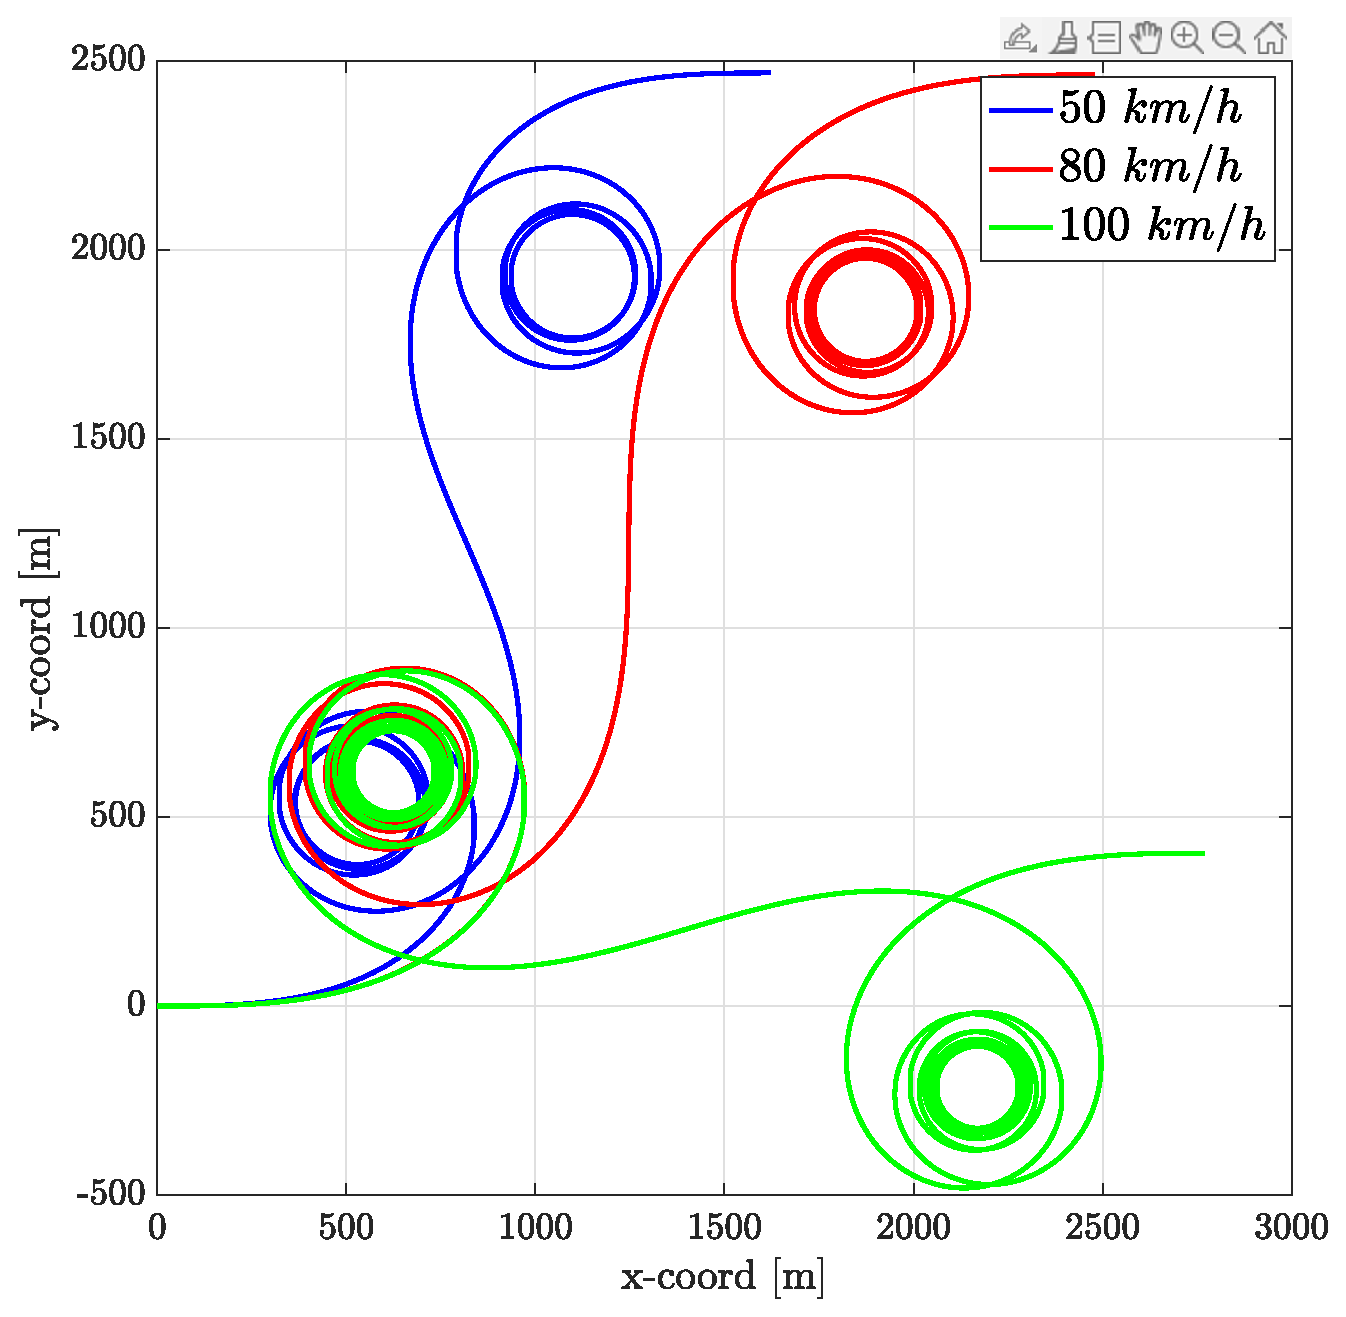
\includegraphics[width=0.75\linewidth]{ex5/q1/ex-51a.eps}
        \centering
        \caption{Vehicle paths for sine steer at different speeds with same $\deltd$}
        \label{51a}
        \end{figure}
        
Plotting the path results of the three different speeds, as shown in Figure \ref{51a}, confirms the over-steering behaviour. The radius of the curvature [the size of the circles] decreases with increasing velocities.

\textbf{Q. carry out other 3 sine steer maneuvers, with these data: \vspace{-1em}
\begin{enumerate}
    \item \boldmath$\deltdz$ = $70^\circ$ , $u$ = 50 km/h
    \item $\deltdz$ = $24^\circ$ , $u$ = 80 km/h
    \item $\deltdz$ = $12^\circ$ , $u$ = 100 km/h
\end{enumerate}}


Figure \ref{52e1} shows the results of maintaining the vehicle's longitudinal velocity $u$ at 50 km/h. A sinusoidal steering maneuver was applied with a large amplitude [$70^\circ$] and a frequency $f$ of $0.001$ $s^{-1}$. This maneuver shows that the vehicle's handling behaviour changes when the lateral acceleration $\ay$ increases above a certain threshold.

The previous runs only had a maximum steering angle of $5^\circ$, which is considered small. With a much bigger maximum steering angle of $70^\circ$, the vehicle exhibits a linear over-steering behaviour while $\ay$ is below 10 $\mss$. Once full saturation is reached, the slope of the curve becomes positive indicating that the behaviour has switched to under-steer.

        \begin{figure}[ht]
        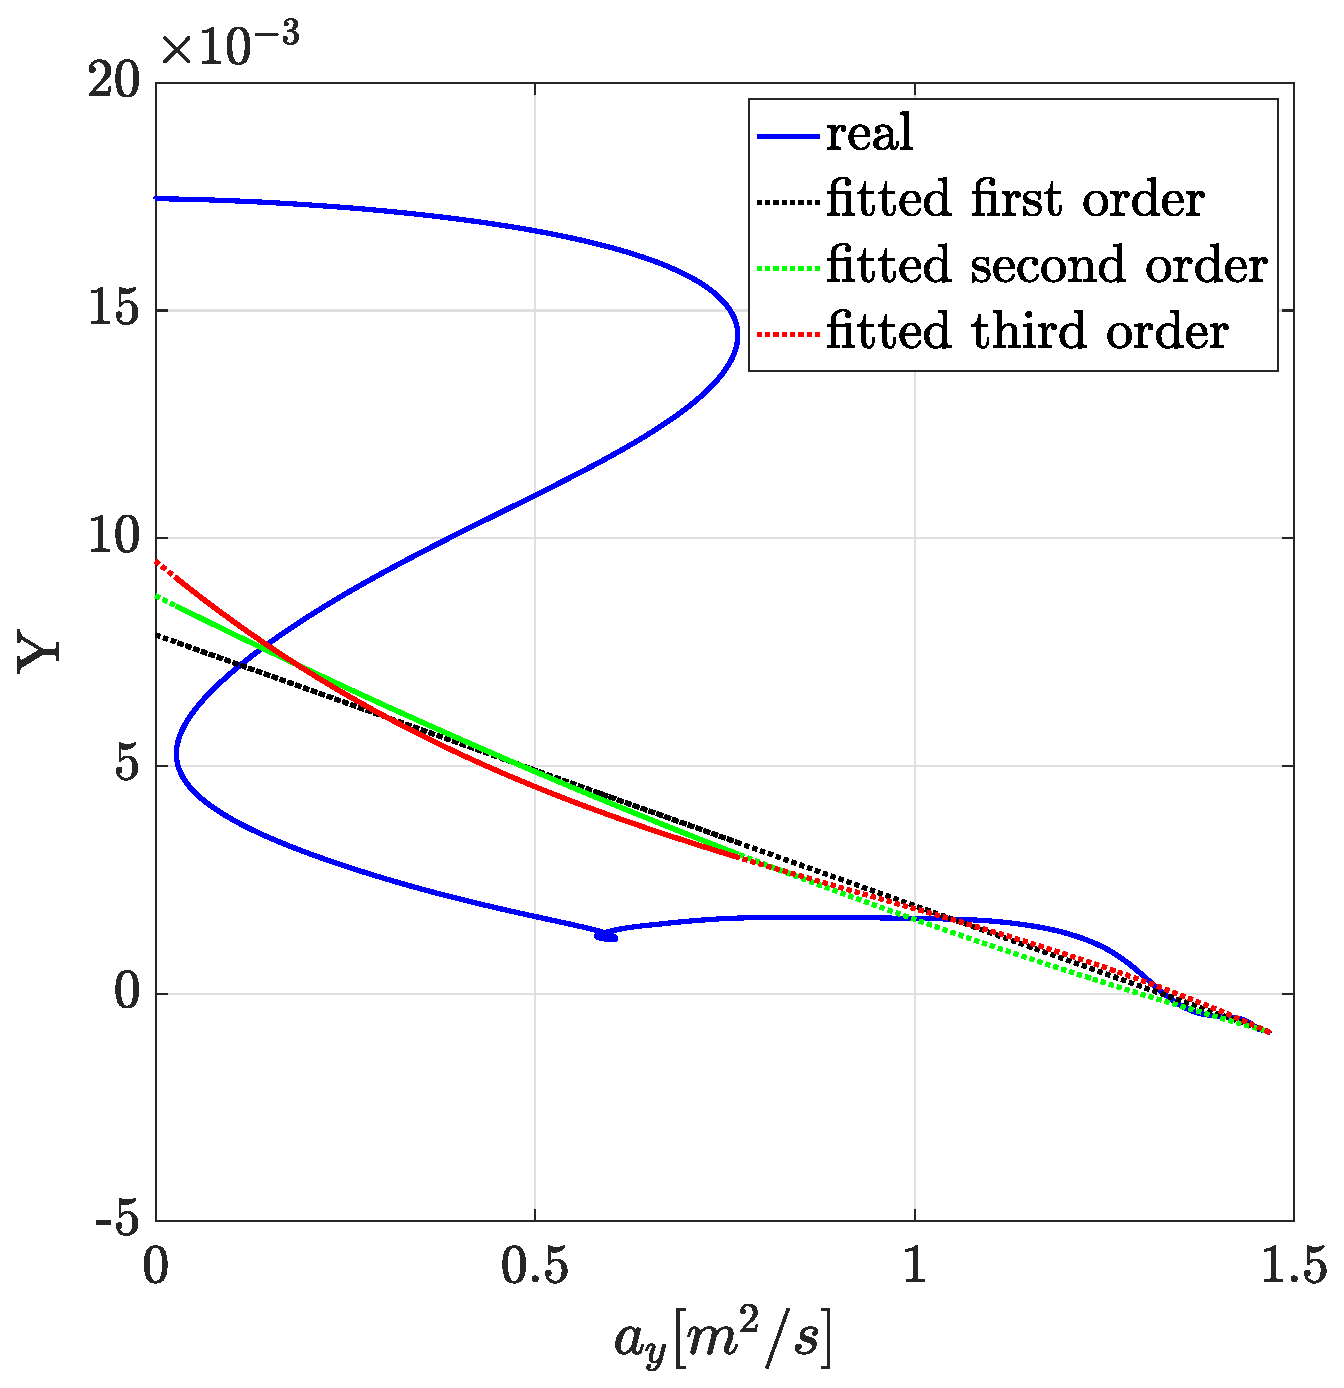
\includegraphics[width=0.75\linewidth]{ex5/q2/ex-52e1.eps}
        \centering
        \caption{Fitted handling diagram result [$\deltdz$\ = $70^\circ$, $u$ = 50 km/h]}
        \label{52e1}
        \end{figure}

The curve can no longer be fitted with a first degree polynomial. Polynomial degrees from one to five were tested, and the lowest and best fitting ones are shown in Figure \ref{52e1}. It appears that a fifth order polynomial is the best approximation for such a curve.

Figures \ref{52e2} and \ref{52e3} show the results of the second and third runs. The effect of higher lateral acceleration $\ay$ on the handling behaviour is not as prevalent in both runs, because the maximum steering angle was much smaller [$12^\circ$ and $24^\circ$ compared to $70^\circ$]. The overall behaviour for the second and third runs stayed as over-steering across $\ay$. However, the curve is not linear. A third order polynomial was the best fitting for both runs. 

        \begin{figure}[ht!]
        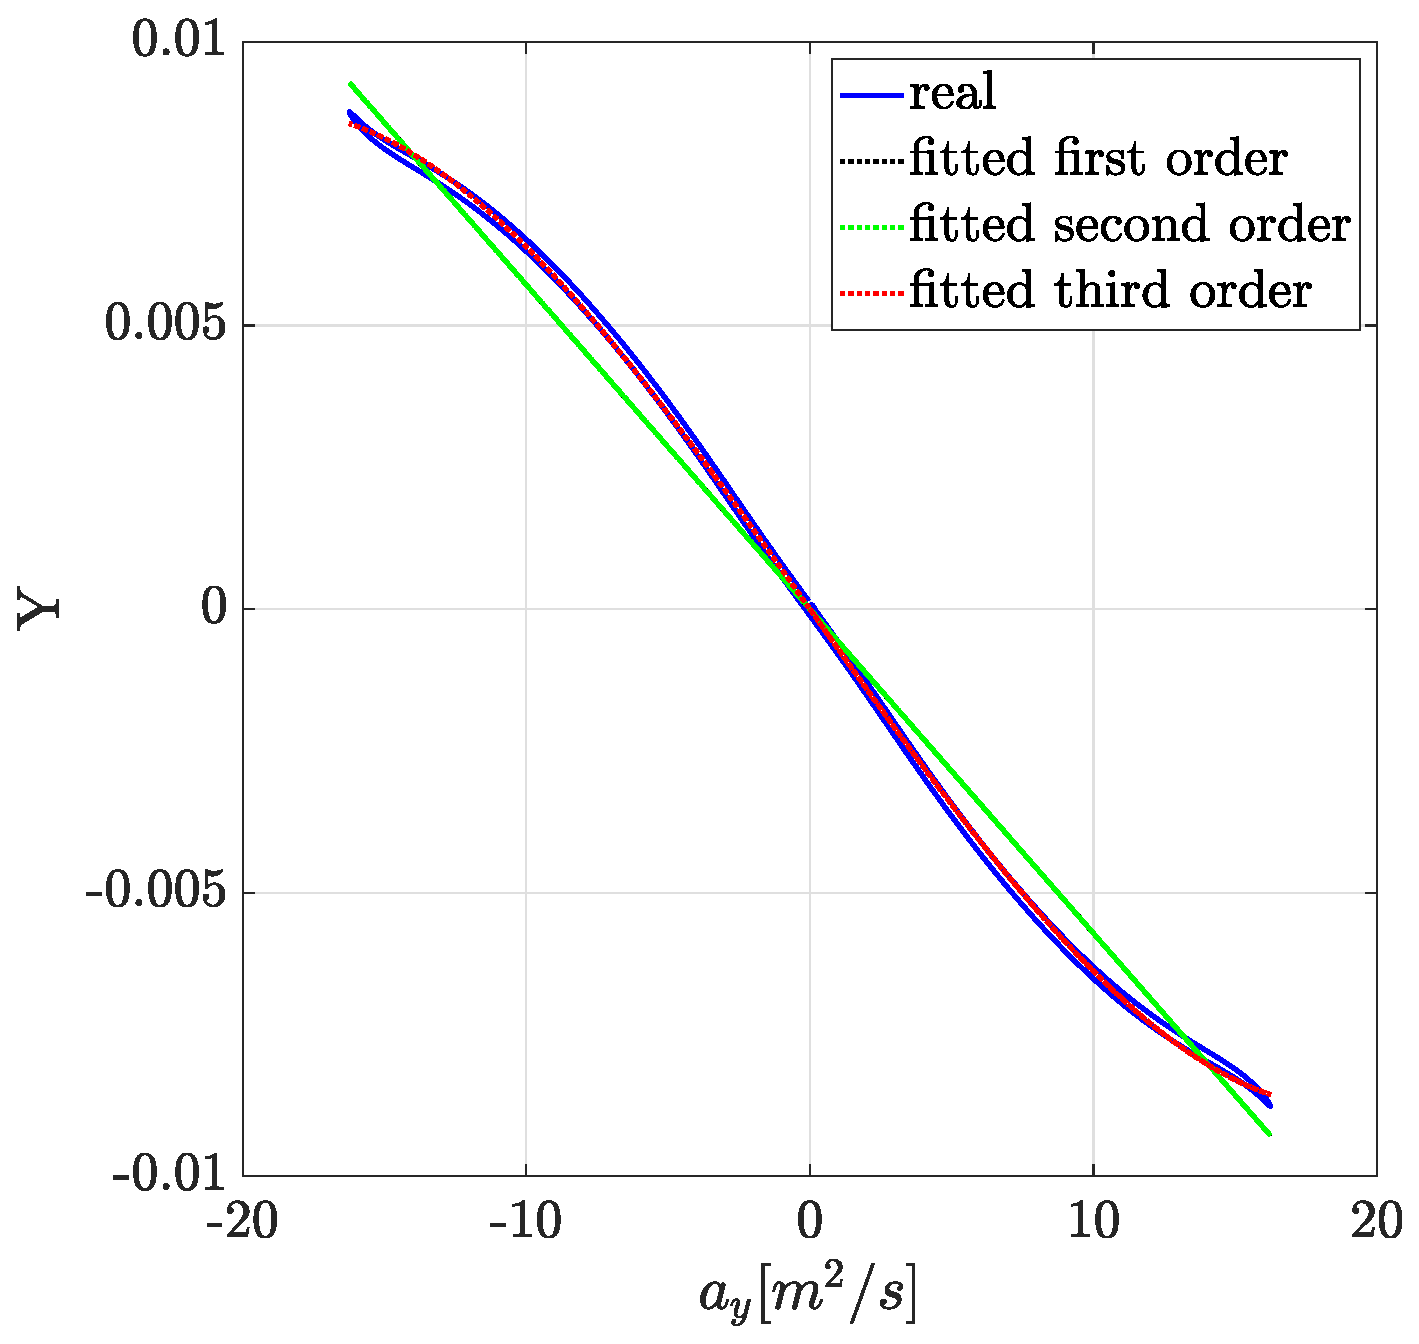
\includegraphics[width=0.63\linewidth]{ex5/q2/ex-52e2.eps}
        \centering
        \caption{Fitted handling diagram result [$\deltdz$\ = $24^\circ$, $u$ = 80 km/h]}
        \label{52e2}
        \end{figure}
        
        \begin{figure}[ht!]
        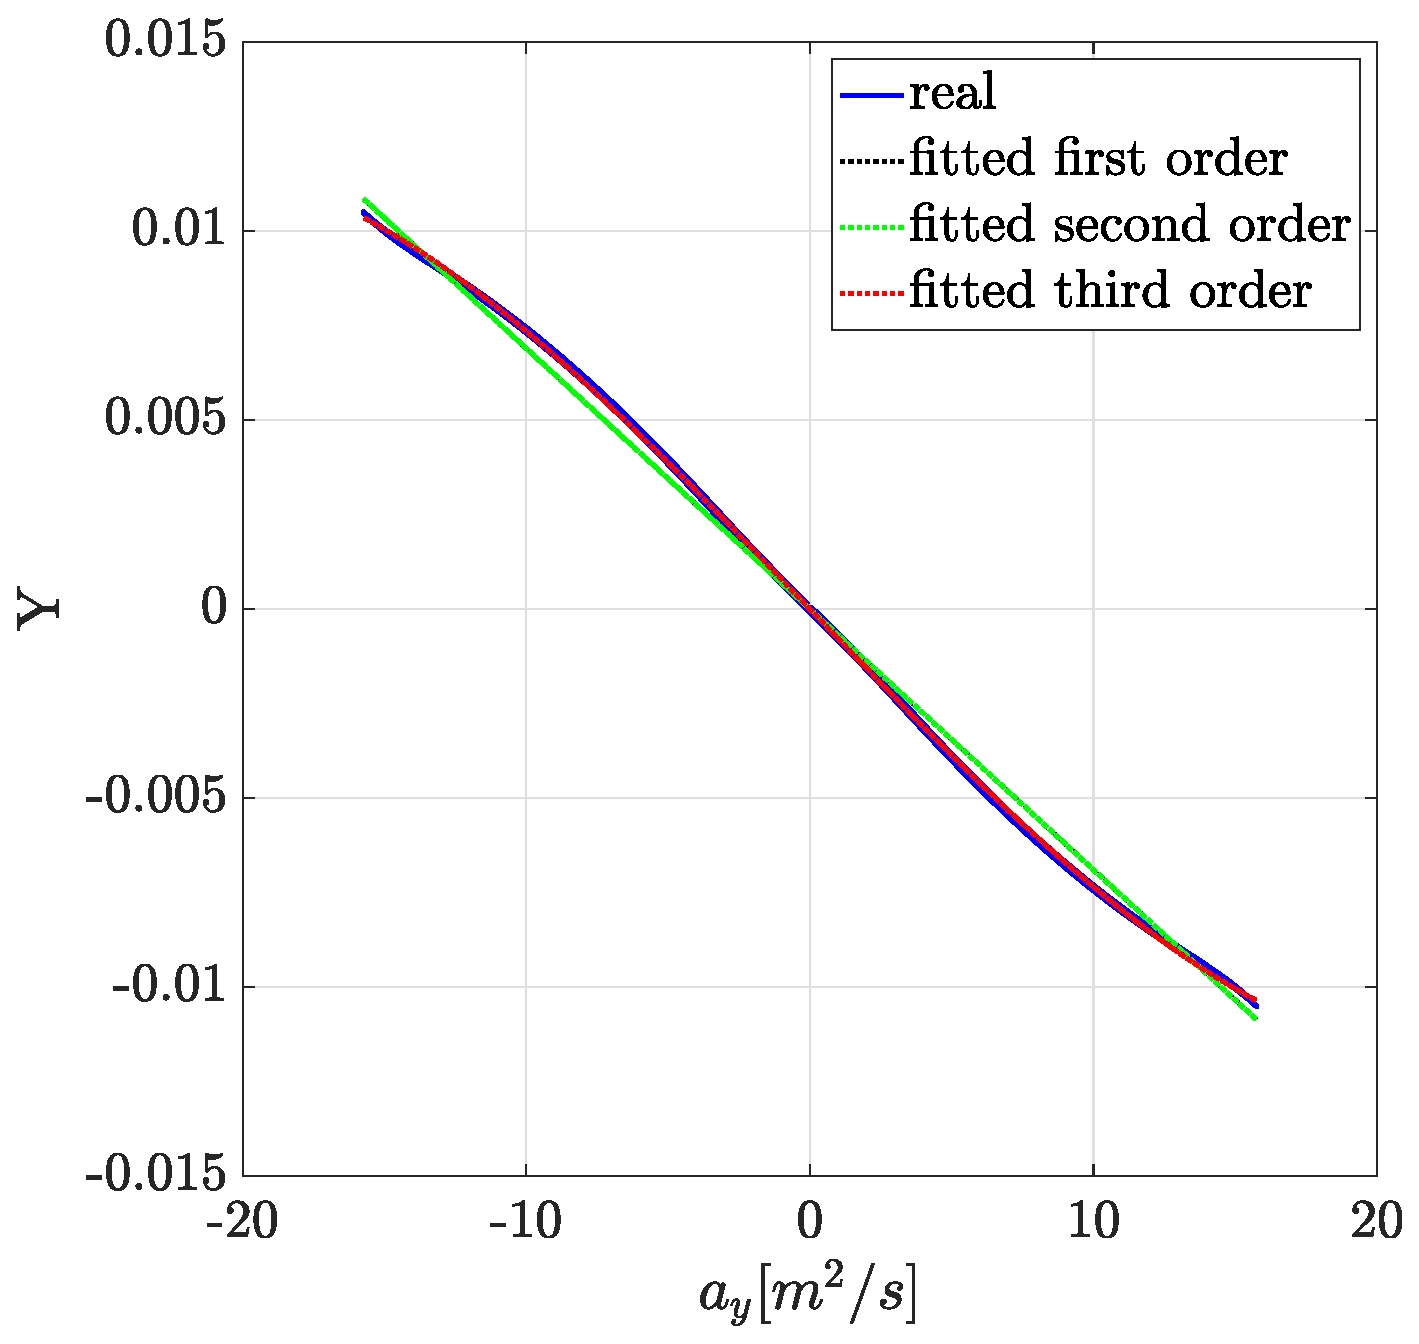
\includegraphics[width=0.63\linewidth]{ex5/q2/ex-52e3.eps}
        \centering
        \caption{Fitted handling diagram result [$\deltdz$\ = $12^\circ$, $u$ = 100 km/h]}
        \label{52e3}
        \end{figure}
        
{\centering\fbox{\begin{minipage}{36em}
\textbf{Coefficients of the polynomial fittings:} \\
run\# 1: [0.0013296, -1.6137e-07, \space0.0003224, \space3.9837e-07, -0.0066391, -1.9657e-07] \\
run\# 2: [0.0010692, \space6.2659e-08, -0.0082143, -9.0719e-08] \\
run\# 3: [0.0007569, \space7.6441e-08, -0.0089127, -8.4754e-08]
\end{minipage}}\par}

The results of all the coefficients for the fittings for the three runs are shown above. They are certainly not constant across the runs because they fit different curves. However, some are quite close, especially runs \# 2 and 3. This could be attributed to the similarity in the linear sections of the three curves as shown in Figure \ref{52d}.

        \begin{figure}[ht]
        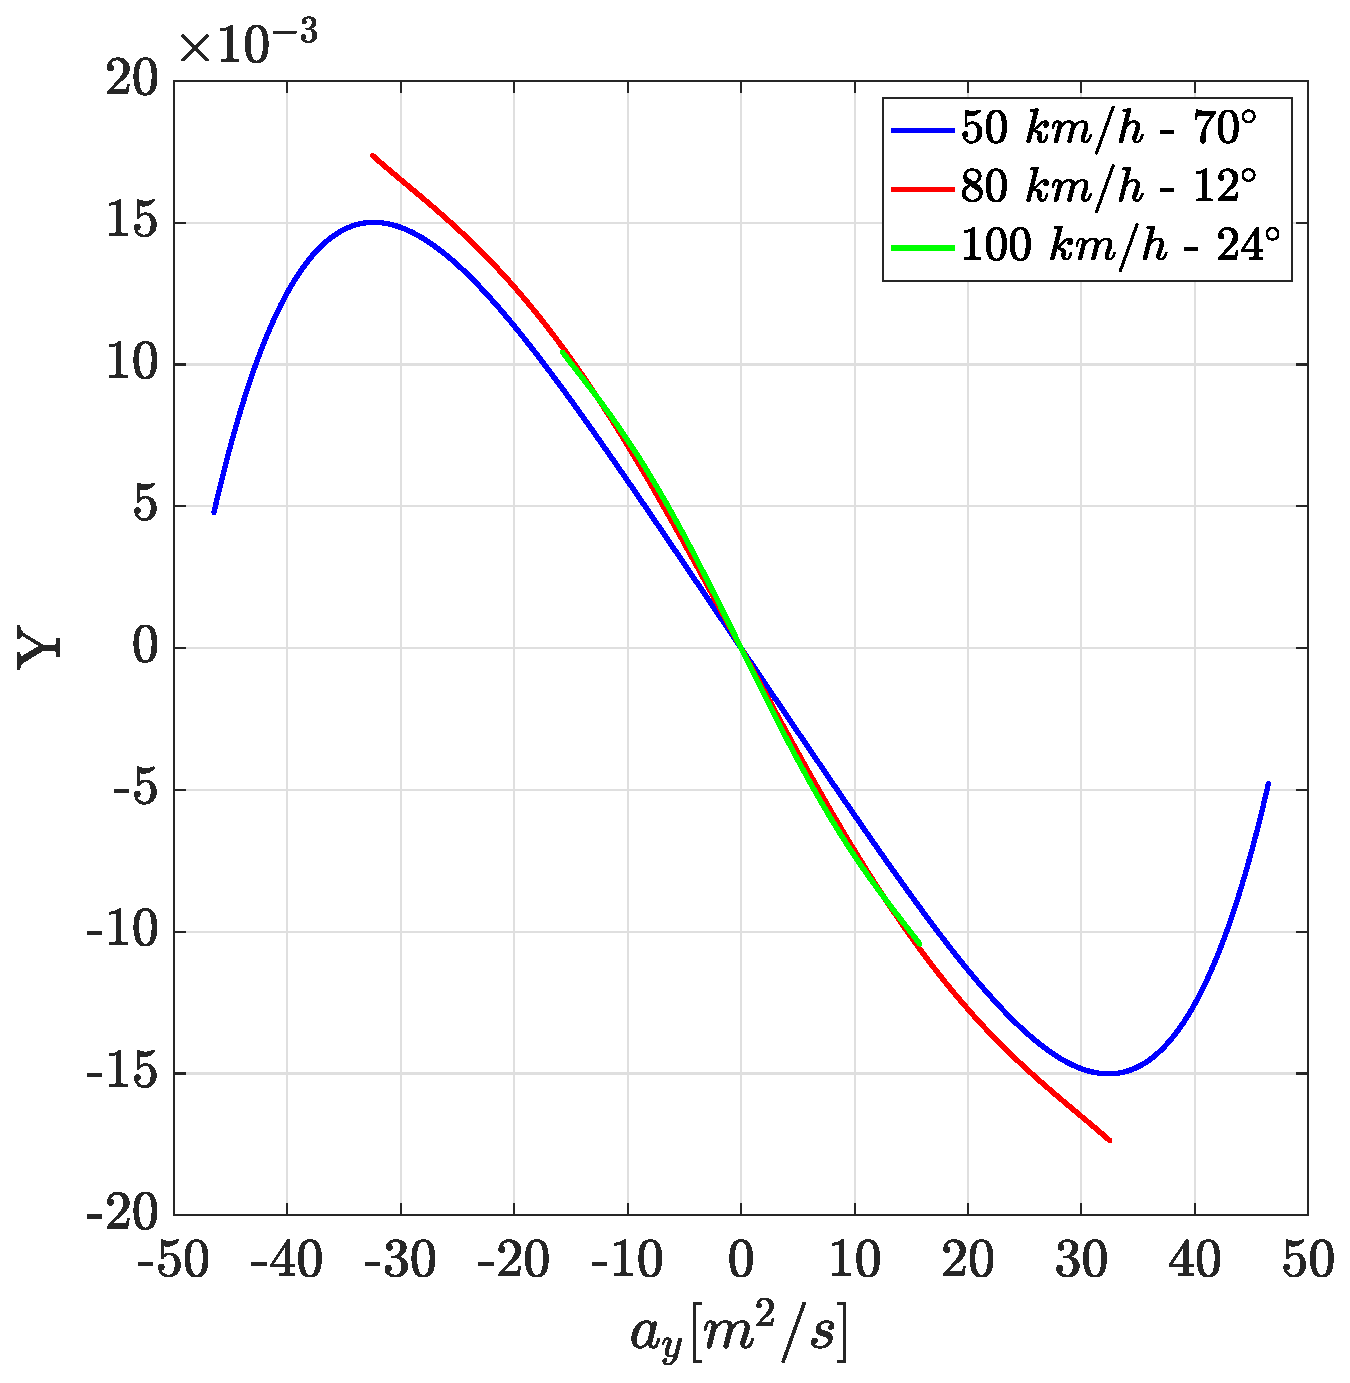
\includegraphics[width=0.7\linewidth]{ex5/q2/ex-52d.eps}
        \centering
        \caption{Fitted handling curves comparison with different $\deltd$}
        \label{52d}
        \end{figure}

\newpage   
\section{Exercise 2 - Constant Steer Maneuvers}
\textbf{Q. Carry out a constant steering maneuver, with these data: \vspace{-1em}
\begin{enumerate}
    \item \boldmath$\deltd$ = $10^\circ$ , $u_{0}$ = 20 km/h , $u_{f}$ = 40 km/h
    \item $\deltd$ = $24^\circ$ , $u_{0}$ = 50 km/h , $u_{f}$ = 80 km/h
\end{enumerate}}

        \begin{figure}[ht]
        
\includegraphics[width=0.99\linewidth]{ex5/q3/ex-53b1.eps}
        \centering
        \caption{Vehicle motion graphs for constant steer maneuver \#1}
        \label{53b1}
        \end{figure}

The simulations were run for 1000 seconds. Figure \ref{53b1} shows the motion graphs for maneuver \#1 [only plotting the first 10 seconds]. The speed ramped up from 20 to 40 km/h within the first 2 seconds using the low level PID controller to manage the pedal.

        \begin{figure}[ht]
        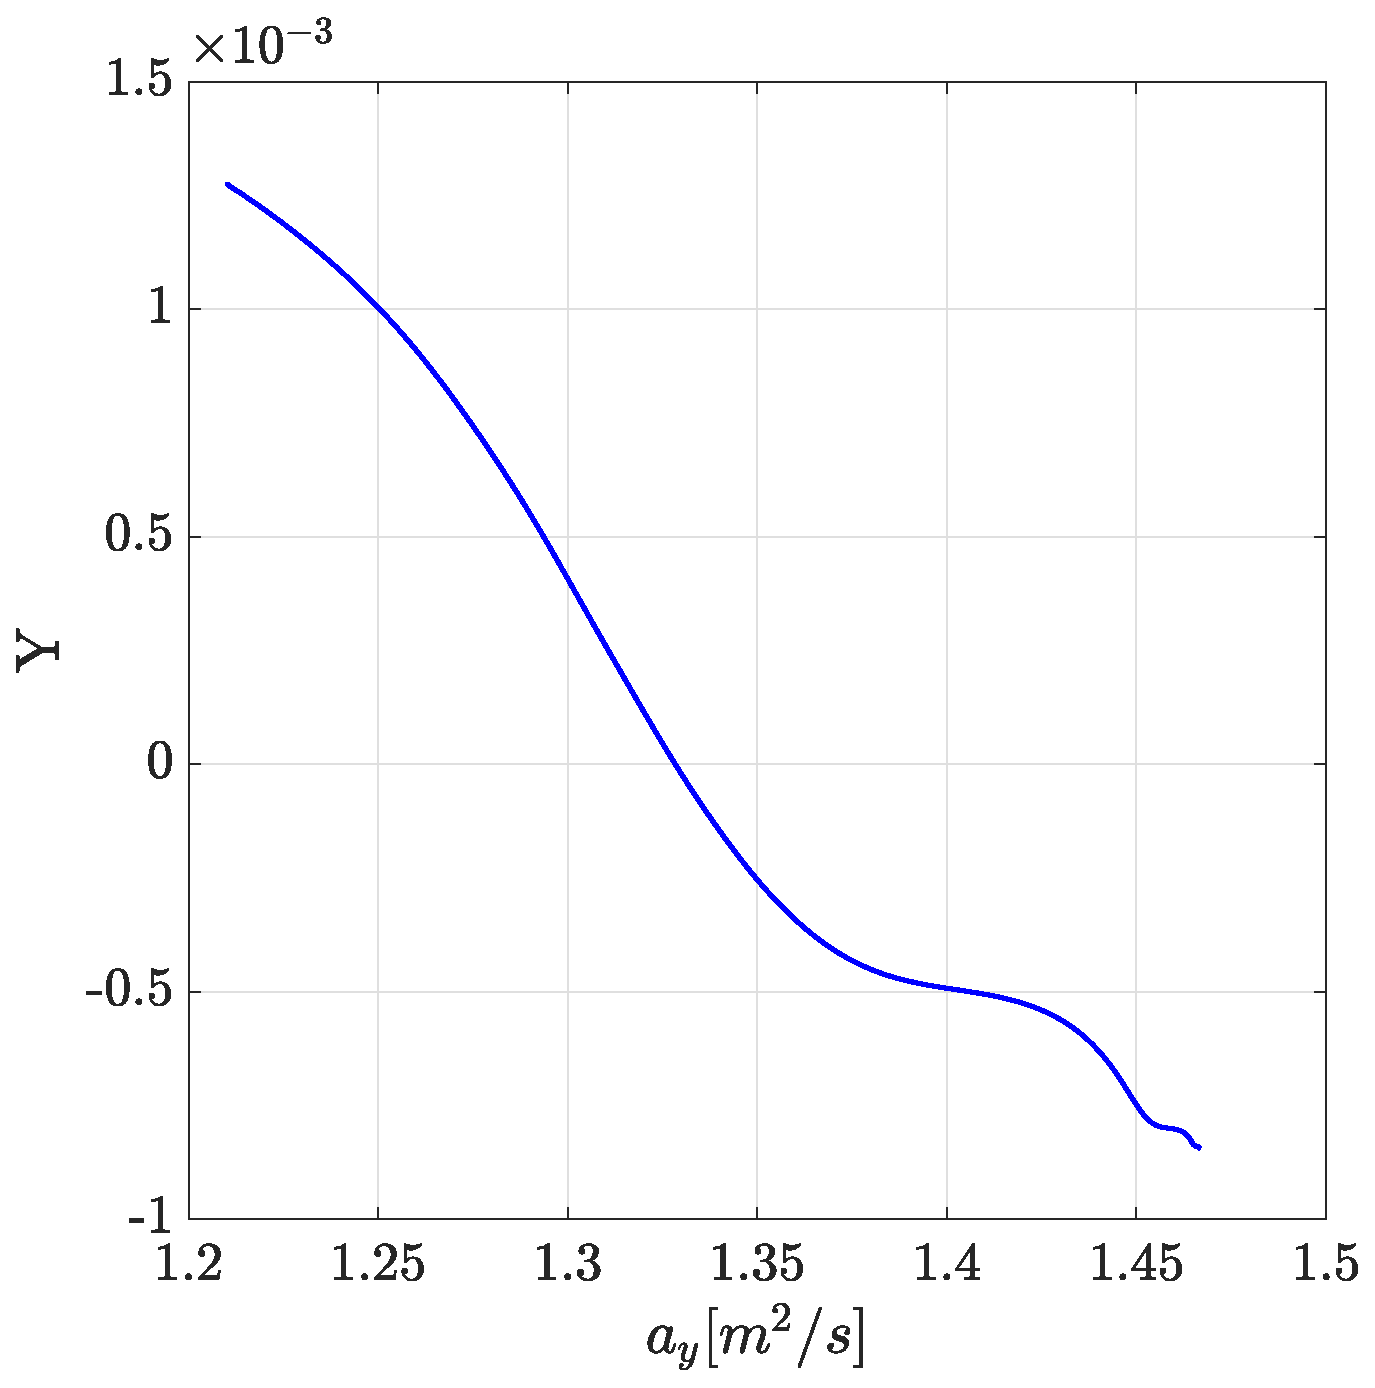
\includegraphics[width=0.37\linewidth]{ex5/q3/ex-53e1.eps}
        \centering
        \caption{Filtered handling curve for constant steer maneuver \#1}
        \label{53e1}
        \end{figure}

The vehicle must be in steady state conditions in order to plot the handling curve. The data was filtered by monitoring the change in $u$ using Equation \ref{eq:5.3a}. The data used in plotting begins at the (steady state start index) till the end [Figure \ref{53e1}].

\begin{equation}\label{eq:5.3a}
\mbox{steady state start index} = \mbox{find ( diff ( $u$ ) )} >= 0.003 m/s
\end{equation}

Even though the filtering has significantly improved the result of the graph, it still is not quite accurate enough. This might be due to the very low lateral acceleration $\ay$ that the vehicle experienced during this maneuver. Nonetheless, the results still suggests that the vehicle has an over-steering behaviour.

The path result of the maneuver plotted in Figure \ref{53m1} shows that the curve was about 80 meters in radius and the vehicle ended almost at the start point. This indicates that the vehicle experienced a negligible amount of over-steer as it was not pushed hard enough to cause any front or rear tire slip. 
        
        
        \begin{figure}[ht]
        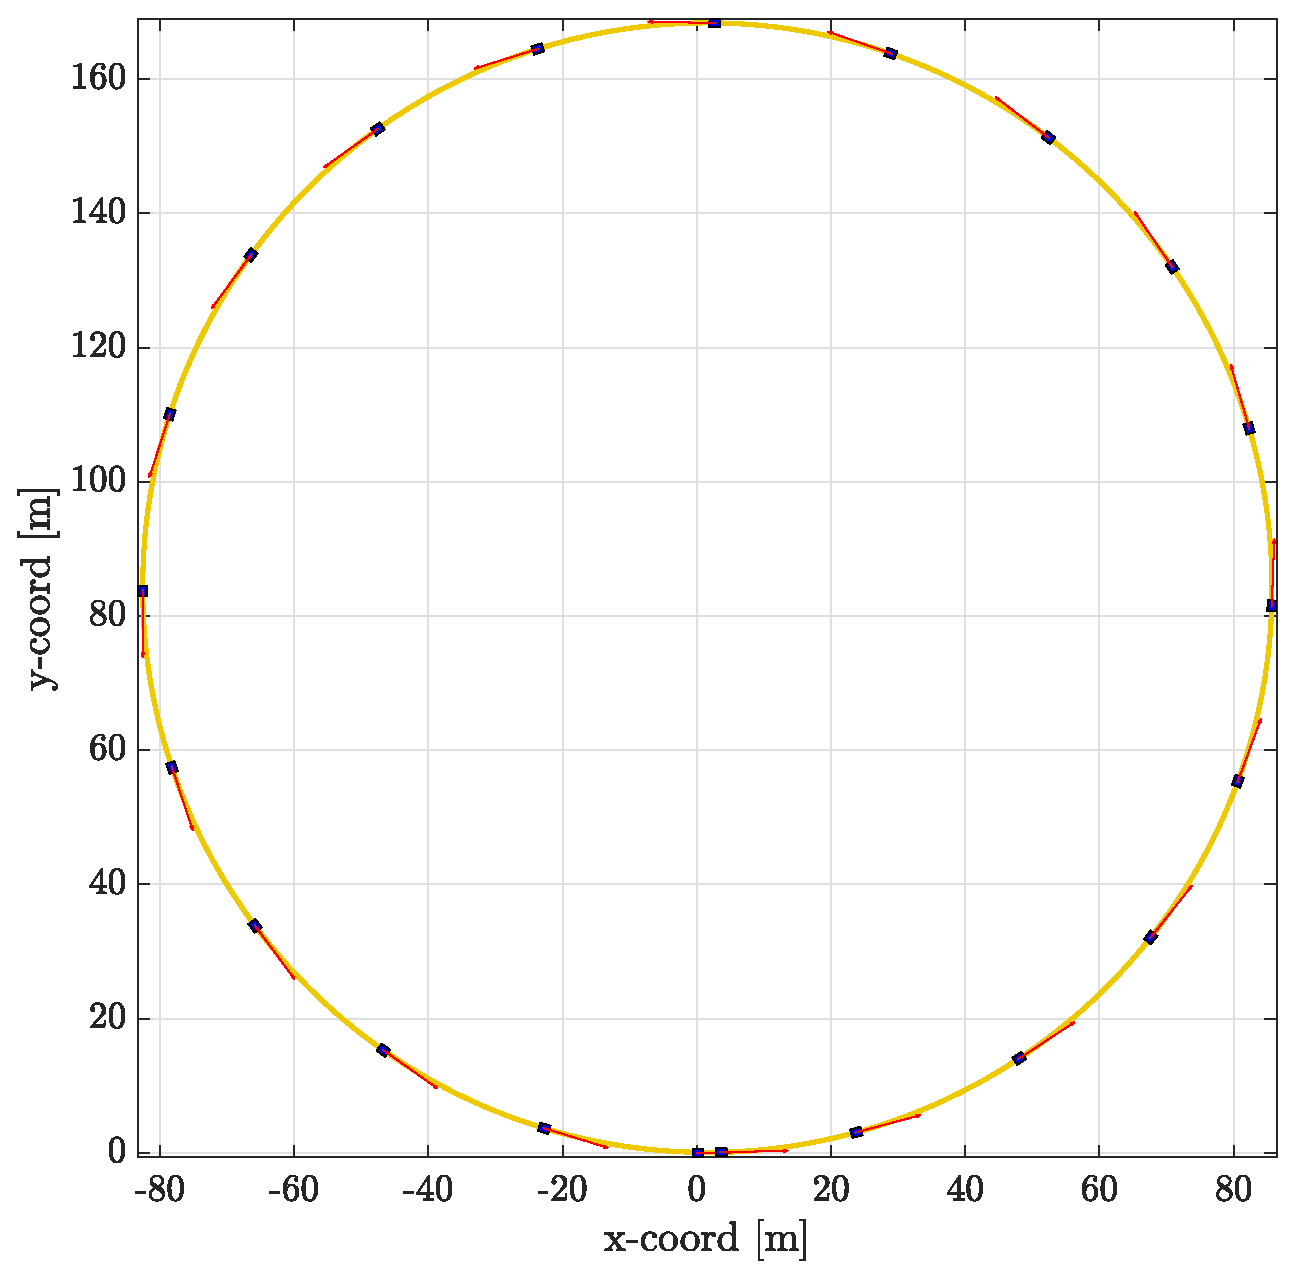
\includegraphics[width=0.5\linewidth]{ex5/q3/ex-53m1.eps}
        \centering
        \caption{Path of the vehicle for constant steer maneuver \#1}
        \label{53m1}
        \end{figure}
        
Similar to maneuver \#1, Figure \ref{53b2} shows the motion graphs for maneuver \#2 [only plotting the first 10 seconds]. The speed ramped up from 40 to 80 km/h within the first 3 seconds using the low level PID controller to manage the pedal.

        \begin{figure}[ht]
        
\includegraphics[width=0.99\linewidth]{ex5/q3/ex-53b2.eps}
        \centering
        \caption{Vehicle motion graphs for constant steer maneuver \#2}
        \label{53b2}
        \end{figure}
        
The filtered handling curve for maneuver \#2 in Figure \ref{53e2} is significantly better than the previous maneuver.  this could be attributed to the much higher lateral acceleration $\ay$ encountered. The curve is almost linear and has a negative slope, which agrees with all the previous maneuvers.


        \begin{figure}[ht]
        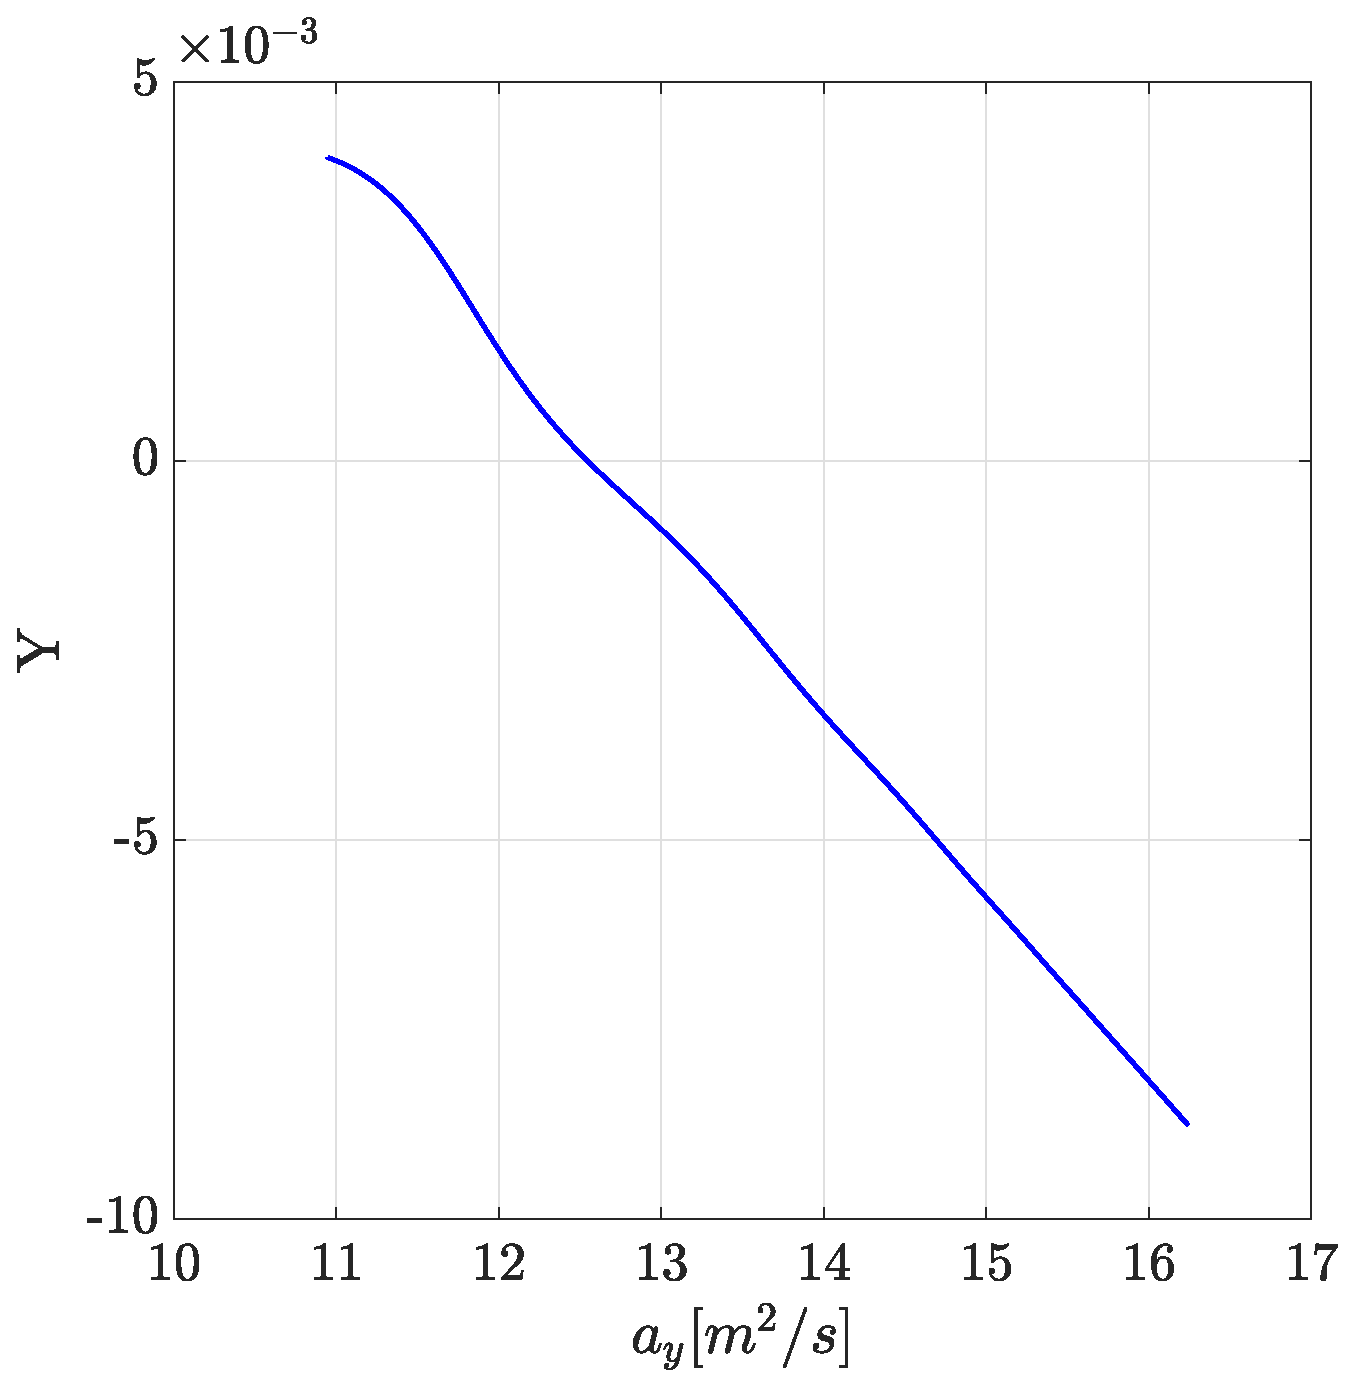
\includegraphics[width=0.4\linewidth]{ex5/q3/ex-53e2.eps}
        \centering
        \caption{Filtered handling curve for constant steer maneuver \#2}
        \label{53e2}
        \end{figure}

The radius of the path with the second maneuver plotted in Figure \ref{53m2} has a much smaller radius [40 meters]. The vehicle has certainly experienced over-steer because the curvature decreased towards the end of the run. 

        \begin{figure}[ht!]
        \includegraphics[width=0.5\linewidth]{ex5/q3/ex-53m2.eps}
        \centering
        \caption{Path of the vehicle for constant steer maneuver \#2}
        \label{53m2}
        \end{figure}